\documentclass[a4paper,german,12pt,smallheadings]{scrartcl}
\usepackage[T1]{fontenc}
\usepackage[utf8]{inputenc}
\usepackage{babel}
\usepackage{tikz}
\usepackage{geometry}
\usepackage{amsmath}
\usepackage{amssymb}
\usepackage{float}
%\usepackage{wrapfig}
\usepackage[thinspace,thinqspace,squaren,textstyle]{SIunits}
\restylefloat{table}
\geometry{a4paper, top=15mm, left=20mm, right=40mm, bottom=20mm, headsep=10mm, footskip=12mm}
\linespread{1.5}
\setlength\parindent{0pt}
\begin{document}
\begin{center}
\bfseries % Fettdruck einschalten
\sffamily % Serifenlose Schrift
\vspace{-40pt}
Elektrodynamik und Optik, Sommersemester 2013, 6/7. Blatt \\
Markus Fenske, Tutor: Dr. Marko Wietstruk
\vspace{-10pt}
\end{center}
\section*{Aufgabe 1}
Das Biot-Savart-Gesetz lautet:

\begin{equation}
  \vec{B}(\vec{r}) = \frac{\mu_0 I}{4 \pi} \int_{\text{Leiter}} \frac{(\vec{r} - \vec{r'}) \times \vec{ds}}{|\vec{r}-\vec{r'}|^3}
\end{equation}

Da hier das Magnetfeld im Ursprung berechnet werden soll, ist:


\begin{equation}
  \vec{B} = \frac{\mu_0 I}{4 \pi} \int_{\text{Leiter}} \frac{(-\vec{r'}) \times \vec{ds}}{|\vec{r'}|^3}
\end{equation}

$\vec{r'}$ ist der der Vektor zum jeweiligen Punkt auf dem Leiter, während
$\vec{ds}$ entlang des Leiters zeigt. Für das gerade Leiterstück ist $\vec{ds}$
also parallel zu $\vec{r}$, womit $\vec{r} \times \vec{ds} = \vec{0}$. Das
gerade Stück kann also vernachlässigt werden.

\begin{equation}
  \vec{B} = \frac{\mu_0 I}{4 \pi} \int_{\text{Bogen}} \frac{(-\vec{r'}) \times \vec{ds}}{|\vec{r'}|^3}
\end{equation}

Auf dem Kreisbogen steht $\vec{ds}$ senkrecht auf $\vec{r}$. Damit gilt dann
$-\vec{r'} \times \vec{ds} = -\widehat{z} (r' ds)$:

\begin{align}
  \vec{B} &= \frac{\mu_0 I}{4 \pi} \int_{\text{Bogen}} -\widehat{z} \frac{r' ds}{r'^3} \\
  \vec{B} &= \frac{\mu_0 I}{4 \pi} \int_{\text{Bogen}} -\widehat{z} \frac{1}{r'^2} ds \\
\end{align}

Sei nun $R$ der Radius des Kreises, dann ist $|\vec{r'}| = R$. Und somit:

\begin{align}
  \vec{B} = -\frac{\mu_0 I}{4 \pi R^2} \widehat{z}\int_{\text{Bogen}} ds \\
\end{align}

Der Kreis hat den Umfang $2 \pi R$, der Halbkreis dementsprechend die Länge
$\pi R$. Das führt zu:

\begin{align}
  \vec{B} = -\frac{\mu_0 I}{4 \pi R^2} \widehat{z} \pi R \\
\end{align}

Und zusammengefasst:

\begin{equation}
  \vec{B} = -\frac{\mu_0 I}{4 \pi R} \widehat{z}
\end{equation}

Da die $z$-Achse aus der Oberseite des Aufgabenblattes herausragt, stimmt dies
auch mit der Rechte-Faust-Regel überein.

\section*{Aufgabe 2}

\begin{figure}[H]
  \begin{center}
    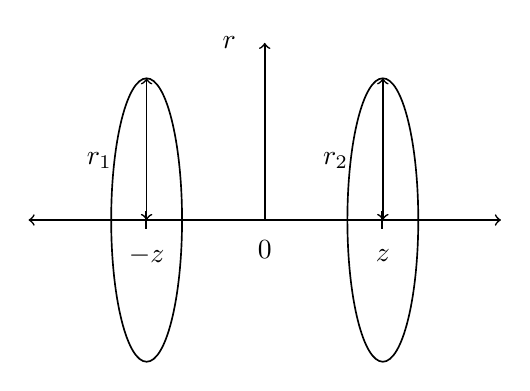
\begin{tikzpicture}[scale=1.5]
      \draw[semithick] (1.0,1.5) ellipse (0.3 and 1.2);% left coil
      \draw[<->,semithick] (1.0,1.5) -- (1.0,2.7); % left radius
      \draw (0.6,2) node {$r_1$}; % left radius text

      \draw[semithick] (3.0,1.5) ellipse (0.3 and 1.2);% right coil
      \draw[<->,semithick] (3.0,1.5) -- (3.0,2.7); % right radius
      \draw (2.6,2) node {$r_2$}; % right radius text

      \draw[->,semithick] (2,1.5) -- (2,3); % r axis
      \draw (1.7,3) node {$r$}; % r axis beschriftung
      \draw (2,1.25) node {$0$}; % ursprung

      \draw[<-|,semithick] (0,1.5) -- (1,1.5);
      \draw[-,semithick] (1,1.5) -- (2,1.5);
      \draw[-|,semithick] (2,1.5) -- (3,1.5);
      \draw[->,semithick] (3,1.5) -- (4,1.5);

      \draw (1,1.2) node {$-z$};
      \draw (3,1.2) node {$z$};
    \end{tikzpicture}
  \end{center}
  \caption{Helmholtzspule}
\end{figure}

Gegeben seien zwei kurze Spulen mit den identischen Radien $r = r_1 = r_2$ und
eine identischen Anzahl an Windungen $N$ an den Positionen $z$ und $-z$. Das
Magnetfeld wird im Zentrum des Aufbaus (also im Ursprung) gemessen und ergibt
sich als Überlagerung der Magnetfelder der beiden Spulen.

Das Magnetfeld einer Leiterschleife ist aus den Vorlesungsunterlagen bekannt,
daher verzichte ich hier auf eine Herleitung. Die Spulen seien Überlagerungen
von jeweils $N$ Leiterschleifen. Daraus folgt für die Magnetfelder:

\begin{align*}
  B = B_1 + B_2 &= \frac{I\mu_0 N}{2} \left(\frac{r^2}{(r^2 + z^2)^{3/2}} + \frac{r^2}{(r^2 + (-z)^2)^{3/2}}\right) \\
            &= I\mu_0 N \left(\frac{r^2}{(r^2 + z^2)^{3/2}}\right)
\end{align*}

Die erste Ableitung lautet:

\begin{align*}
  \frac{\partial B}{\partial z} &= I\mu_0 N  r^2 \left(-\frac{3}{2}\right) \cdot 2z \cdot \frac{1}{(r^2 + z^2)^{5/2}} \\
                                &= I\mu_0 N \frac{-3zr^2}{(r^2 + z^2)^{5/2}}
\end{align*}

Die zweite Ableitung lautet:

\begin{align*}
  \frac{\partial^2 B}{\partial z^2} &= -I\mu_0 N \cdot 3 r^2 \frac{\partial}{\partial z} \frac{z}{(r^2 + z^2)^{5/2}} \\
                                    &= -I\mu_0 N \cdot 3 r^2 \left(\frac{1}{(r^2 + z^2)^{5/2}} - \frac{5z^2}{(r^2+z^2)^{7/2}}\right) \\
                                    &= -I\mu_0 N \cdot 3 r^2 \frac{1}{(r^2 + z^2)^{7/2}} \left( (r^2+z^2) - 5z^2 \right) \\
                                    &= -I\mu_0 N \cdot 3 r^2 \frac{1}{(r^2 + z^2)^{7/2}} \left( r^2 - 4z^2 \right) \\
\end{align*}

Die zweite Ableitung nun weiter zusammenzufassen wäre Verschwendung von
teurer Drucktinte. Wir suchen $\partial_z^2 B \overset{!}{=} 0$. Obiger Ausdruck
muss also null werden. Dies passiert offensichtlich nur dann, wenn die innerste
Klammer null wird.

\begin{align*}
  &r^2 - 4z^2 \overset{!}{=} 0 \\
  \Leftrightarrow\quad & r^2 = 4z^2 \\
  \Leftrightarrow\quad & r =  \pm 2z \\
  \Rightarrow\quad &z = \pm\frac{r}{2}
\end{align*}

Die Abstände $z$ müssen also jeweils das Halbe des Spulenradius betragen,
damit das Feld möglichst homogen wird. Das $\pm$ bedeutet nur, dass die Spulen
prinzipiell vertauschbar sind. Der Abstand zwischen den Spulen muss also genau
dem Radius der Spulen entsprechen.

\section*{Aufgabe 3}

\begin{equation}
  \vec{p}_m = I \vec{A}
\end{equation}

Das magnetische Dipolmoment ist $p_m = I \cdot \vec{A}$. Dabei ist $I$ der
Strom und $\vec{A}$ die Flächennormale der Kreisbahn. Da diese parallel zum
Drehmoment, genau wie zum Drehimpuls ist, reicht es, hier mit Beträgen zu
arbeiten.

\begin{equation}
  p_m = I A
\end{equation}

Für $I$ gilt $I = \frac{dQ}{dt}$. Das Elektron kommt auf seiner Kreisbahn mit
dem Radius $r$ genau einmal pro Umlaufzeit $t$ am Ausgangspunkt vorbei. Der
Strom ist also

\begin{equation}
  I = \frac{-e}{t}
\end{equation}

Die Umlaufzeit auf der Kreisbahn $s$ mit der Geschwindigkeit $v$ ist:

\begin{equation}
  t = \frac{s}{v} = \frac{2 \pi r}{v}
\end{equation}

Eingesetz in die Ausgangsgleichung:

\begin{equation}
  p_m = \frac{-e}{2 \pi r} v A
\end{equation}

Die Kreisfläche ist $A = \pi r^2$. Eingesetzt:

\begin{equation}
  p_m = \frac{-e}{2 \pi r} v \pi r^2 = \frac{-e}{2} v r
\end{equation}

Mit dem Impuls $p = mv$ erhält man:

\begin{equation}
  p_m = \frac{-e}{2m} p r
\end{equation}

Und mit dem Drehimpulsbetrag $L = pr$:

\begin{equation}
  p_m = \frac{-e}{2m} L
\end{equation}

Wenn ich nun $L = \hbar$ einsetze erhalte ich:

\begin{equation}
  p_m = \frac{-e}{2m_e} \hbar \approx -9{,}274 \cdot 10^{-24} \;\joule\per\tesla
\end{equation}

\section*{Aufgabe 7}
\subsection*{Teil a}
Für das Magnetfeld einer langen Spule gilt

\begin{equation}
  B = \mu_0 \mu_r \frac{n}{l} I
\end{equation}

In diesem Fall:

\begin{align*}
  B \approx 60 \;\milli\tesla
\end{align*}

\subsection*{Teil b}
Aus obiger Gleichung ist klar, dass $I$ mit dem Faktor $1200$ multipliziert
werden muss, wenn $\mu$ durch $1200$ dividiert wird. Dementsprechend muss dann
$I = 1200 \cdot 20\;\milli\ampere = 24\;\ampere$ sein.



\end{document}
